\documentclass{article}
\usepackage[T2A]{fontenc}

\usepackage[]{graphicx}
\usepackage{float}
\usepackage{amsmath,amsthm,amssymb,amsfonts}
\usepackage{color}

\begin{document}
\section{Радиус описанной окружности правильного многоугольника, формула}

% section * (end)
\begin{figure}[H]
 \begin{center}
  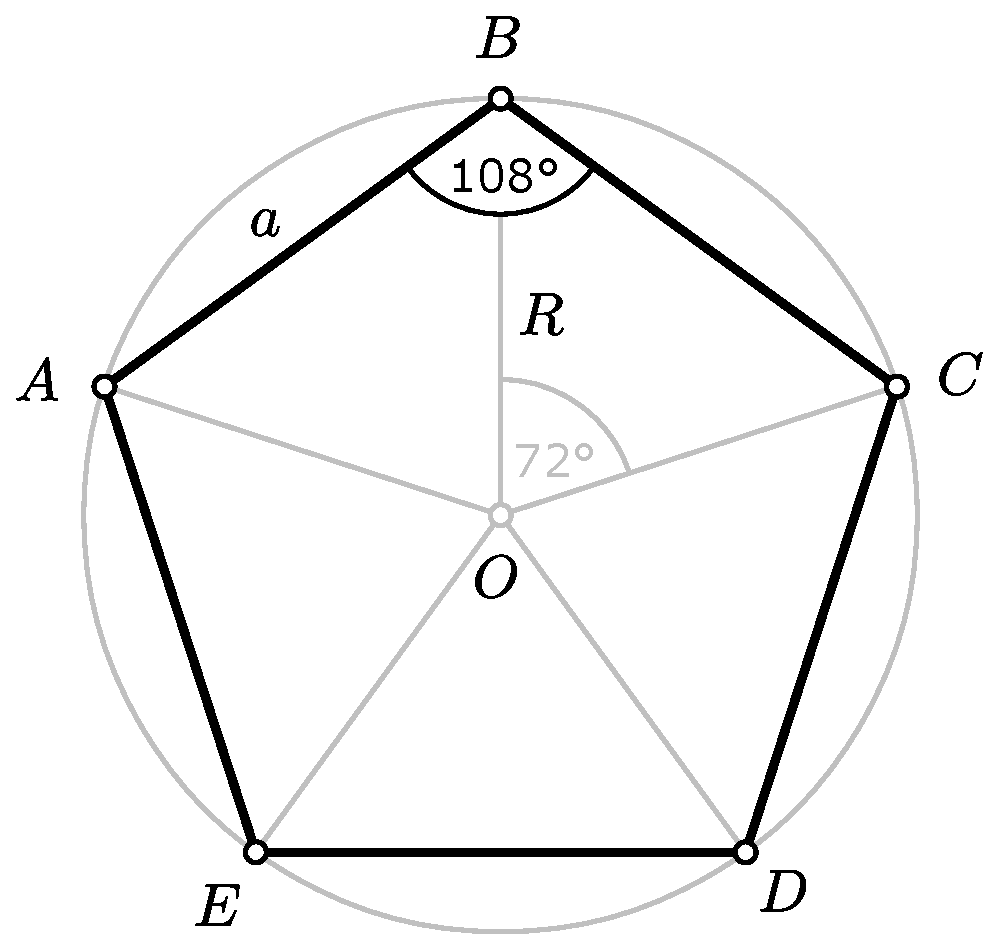
\includegraphics[width=.4\textwidth]{regular_polygon_5_annotated.eps}
 \end{center}
 \caption{Regular polygon}
 \label{fig:regular_polygon_5_annotated}
\end{figure}
Правильный многоугольник -- это многоугольник с равными сторонами и углами. Угол 
между двумя соседними вершинами правильного $n$-угольника равен:

\begin{equation}\label{eq:angle}
  \angle AOB = \frac{360}{n}.
\end{equation}

Построим треугольник $\triangle AOB$ отдельно. Об этом треугольнике мы знаем: он 
равнобедренный, и бедра этого треугольника это радиусы описанной окружности 
правильного многоугольника. Также нам известна длина осно\-вания $a$ этого 
треугольника -- которое является стороной исходного пра\-вильного многоугольника.

\begin{figure}[H]
 \begin{center}
  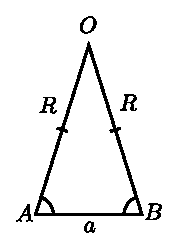
\includegraphics[width=.2\textwidth]{./triangle.eps}
 \end{center}
 \caption{Triangle}
 \label{fig:triangle}
\end{figure}

Также известен угол между радиусами $R$ -- по формуле~\eqref{eq:angle}. Опустим 
высоту на 
основание и рассмотрим получившийся прямоугольный треугольник. При помощи 
тригонометрических функций острого угла получим:
\begin{equation}\label{eq:sin}
  \sin \left( \frac{360^{\circ}}{2n} \right)
  = \frac{a}{2R}.
\end{equation}
отсюда получим формулу 
\textbf{радиуса описанной окружности правильного многоугольника}:
\begin{equation}\label{eq:result}
  R = \frac{a}{2\sin \frac{360^{\circ}}{2n}},
\end{equation}

где $a$ -- сторонa правильного многоугольника; $n$ -- число сторон правильного 
многоугольника; $R$ - радиус описанной окружности правильного многоугольника.


\end{document}
